% ===================================================================
%  Week 10 — Feature Detection & Matching
% ===================================================================
\documentclass[10pt,aspectratio=169]{beamer}
% ===================================================================
%  Shared Beamer preamble for "Practical Image Processing"
%  English slides. Compile with pdfLaTeX.
% ===================================================================

\usetheme{metropolis}
\usepackage[T1]{fontenc}
\usepackage[utf8]{inputenc}
\usepackage{lmodern}
\usepackage{listings}
\usepackage{tcolorbox}
\usepackage{fontawesome5}
\usepackage{booktabs}
\usepackage{amsmath,amssymb}
\usepackage{tikz}
\usepackage{pgfplots}
\pgfplotsset{compat=1.17}
\usetikzlibrary{arrows.meta,positioning,shapes.geometric,fit,backgrounds,matrix}
\tcbuselibrary{skins,breakable}

% ---- Palette --------------------------------------------------------
\definecolor{coursePrimary}{HTML}{1B4965}   % deep blue
\definecolor{courseAccent}{HTML}{E76F51}    % coral
\definecolor{courseGood}{HTML}{2A9D8F}      % teal
\definecolor{courseBad}{HTML}{C0392B}       % red
\definecolor{courseInfo}{HTML}{2980B9}      % blue
\definecolor{codeBg}{HTML}{F5F6FA}
\definecolor{codeKw}{HTML}{8E44AD}
\definecolor{codeStr}{HTML}{2A9D8F}
\definecolor{codeCom}{HTML}{7F8C8D}

\setbeamercolor{frametitle}{bg=coursePrimary}
\setbeamercolor{progress bar}{fg=courseAccent}
\setbeamercolor{alerted text}{fg=courseAccent}
\metroset{block=fill,sectionpage=progressbar,numbering=fraction}

% ---- Code listings (Python is built into listings) -----------------
\lstdefinestyle{course}{
  backgroundcolor=\color{codeBg},
  basicstyle=\ttfamily\scriptsize,
  keywordstyle=\color{codeKw}\bfseries,
  stringstyle=\color{codeStr},
  commentstyle=\color{codeCom}\itshape,
  numberstyle=\tiny\color{codeCom},
  numbers=left, numbersep=6pt,
  showstringspaces=false, breaklines=true, breakatwhitespace=true,
  tabsize=4, columns=fullflexible,
  frame=single, framesep=4pt, rulecolor=\color{gray!30},
  keepspaces=true, upquote=true, language=Python,
}
\lstset{style=course}
\lstdefinelanguage{bash}{
  keywords={cd,pip,python,venv,source,import}, sensitive=true,
  morecomment=[l]{\#}, morestring=[b]', morestring=[b]",
}

% ---- Reusable callout boxes ----------------------------------------
\newtcolorbox{goodbox}[1][Good practice]{colback=courseGood!8,colframe=courseGood,
  fonttitle=\bfseries,title={\faCheck~#1},boxrule=0.6pt,left=4pt,right=4pt,top=3pt,bottom=3pt}
\newtcolorbox{badbox}[1][Pitfall]{colback=courseBad!8,colframe=courseBad,
  fonttitle=\bfseries,title={\faTimes~#1},boxrule=0.6pt,left=4pt,right=4pt,top=3pt,bottom=3pt}
\newtcolorbox{infobox}[1][Note]{colback=courseInfo!8,colframe=courseInfo,
  fonttitle=\bfseries,title={\faInfoCircle~#1},boxrule=0.6pt,left=4pt,right=4pt,top=3pt,bottom=3pt}
\newtcolorbox{mathbox}[1][Math]{colback=coursePrimary!6,colframe=coursePrimary,
  fonttitle=\bfseries,title={\faCalculator~#1},boxrule=0.6pt,left=4pt,right=4pt,top=3pt,bottom=3pt}

\newcommand{\keyidea}[1]{\begin{alertblock}{Key idea}#1\end{alertblock}}
\newcommand{\term}[1]{\textbf{\color{coursePrimary}#1}}
\newcommand{\code}[1]{\lstinline[basicstyle=\ttfamily\small]|#1|}

% ---- A helper to draw a small pixel grid, cells shaded by value ----
% \pixelgrid{ {10,20,120,200,240}, {30,60,130,180,230}, ... }
\newcommand{\pixelgrid}[1]{%
  \begin{tikzpicture}[font=\scriptsize,scale=0.6]
    \foreach \row [count=\ry] in {#1} {
      \foreach \val [count=\cx] in \row {
        \draw[gray,fill=coursePrimary!8] (\cx,-\ry) rectangle ++(1,-1);
        \node at (\cx+0.5,-\ry-0.5) {\val};
      }
    }
  \end{tikzpicture}}


\title{Feature Detection \& Matching}
\subtitle{Week 10 — Finding and comparing distinctive points}
\author{Practical Image Processing}
\date{Lecture 10 \textbullet\ 60--70 min}

\begin{document}

\maketitle

\begin{frame}{Recap \& today}
  \begin{columns}[T]
    \begin{column}{0.58\textwidth}
      \begin{itemize}
        \item Wk5--9: edges, regions, shapes — describing an image's content.
        \item \alert{Today:} \term{features} — distinctive points (corners) with \term{descriptors}
              you can \term{match} across images, even under rotation and scale.
      \end{itemize}
    \end{column}
    \begin{column}{0.42\textwidth}
      \begin{alertblock}{DocScan milestone}
        Matching features between a photographed page and a template lets us align/rectify it —
        the setup for Week 11's perspective correction.
      \end{alertblock}
    \end{column}
  \end{columns}
\end{frame}

\begin{frame}{Roadmap}\tableofcontents\end{frame}

% ==================================================================
\section{Corners: what makes a good feature}
% ==================================================================

\begin{frame}{What is a good feature point?}
  \begin{itemize}
    \item \term{Distinctive}: it looks different from its surroundings (so it can be found again).
    \item \term{Repeatable}: the same physical point is detected across images (different view/light).
    \item \term{Local}: described by a small patch, robust to partial occlusion.
  \end{itemize}
  \keyidea{Flat regions and straight edges are ambiguous; \term{corners} are the classic good feature — they pin down a location in 2D.}
\end{frame}

\begin{frame}{Flat / edge / corner}
  \begin{itemize}
    \item \term{Flat} patch: moving it any direction looks the same $\rightarrow$ no localization.
    \item \term{Edge}: moving \emph{along} the edge looks the same $\rightarrow$ 1D ambiguity.
    \item \term{Corner}: moving \emph{any} direction changes the patch $\rightarrow$ pinned in 2D.
  \end{itemize}
  \begin{mathbox}
    The \term{Harris} detector measures intensity change in all directions via the structure matrix's eigenvalues.
  \end{mathbox}
\end{frame}

\begin{frame}{Harris corners — on a real car}
  \begin{columns}[T]
    \begin{column}{0.5\textwidth}\begin{center}
      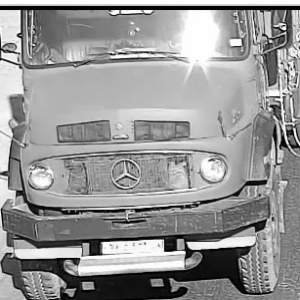
\includegraphics[width=0.9\linewidth]{../assets/gray.png}\\{\scriptsize grayscale}
    \end{center}\end{column}
    \begin{column}{0.5\textwidth}\begin{center}
      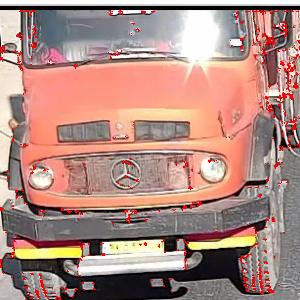
\includegraphics[width=0.9\linewidth]{../assets/harris.png}\\{\scriptsize Harris corners (red)}
    \end{center}\end{column}
  \end{columns}
  \vspace{3pt}
  Corners land on distinctive junctions (lights, edges of parts) — repeatable points to match on.
\end{frame}

\begin{frame}{The structure matrix, intuitively}
  \begin{itemize}
    \item Look at how image gradients $(I_x, I_y)$ vary inside a small window.
    \item Build the $2\times2$ matrix $M=\sum \left(\begin{smallmatrix} I_x^2 & I_xI_y \\ I_xI_y & I_y^2 \end{smallmatrix}\right)$.
    \item Its two eigenvalues $\lambda_1,\lambda_2$ say how much the patch changes in the two principal directions.
  \end{itemize}
  \begin{mathbox}
    Both small $\rightarrow$ flat. One large $\rightarrow$ edge. \alert{Both large $\rightarrow$ corner.}
    Harris score $R=\lambda_1\lambda_2-k(\lambda_1+\lambda_2)^2$ avoids computing eigenvalues directly.
  \end{mathbox}
\end{frame}

\begin{frame}{Corner detectors}
  \begin{center}
  \begin{tabular}{@{}lll@{}}
    \toprule
    \textbf{Detector} & \textbf{Idea} & \textbf{Note} \\
    \midrule
    Harris & eigenvalues of structure matrix & classic, accurate \\
    Shi-Tomasi & min eigenvalue (goodFeaturesToTrack) & great for tracking \\
    FAST & pixel-ring intensity test & very fast, used in ORB \\
    \bottomrule
  \end{tabular}
  \end{center}
  \keyidea{Detecting \emph{where} the feature is (the keypoint) is step one. Describing \emph{what it looks like} (the descriptor) is step two.}
\end{frame}

% ==================================================================
\section{Descriptors}
% ==================================================================

\begin{frame}{From keypoint to descriptor}
  \begin{itemize}
    \item A \term{descriptor} is a vector summarizing the patch around a keypoint.
    \item Good descriptors are \term{invariant}: same value under rotation, scale, and lighting change.
    \item Match two images by finding keypoints with \emph{similar descriptors}.
  \end{itemize}
  \begin{mathbox}
    SIFT: a 128-D vector of gradient-orientation histograms; robust to rotation/scale/illumination.
  \end{mathbox}
\end{frame}

\begin{frame}{ORB keypoints — on the real car}
  \begin{center}
  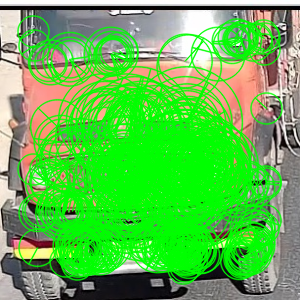
\includegraphics[width=0.55\linewidth]{../assets/orb_keypoints.png}
  \end{center}
  \begin{itemize}
    \item \term{ORB} = FAST keypoints + BRIEF descriptor, made rotation-aware. Free and fast.
    \item Each circle: a keypoint with a size (scale) and orientation.
    \item 380 keypoints here — each a distinctive point with a binary descriptor to match.
  \end{itemize}
\end{frame}

\begin{frame}{SIFT vs ORB (and friends)}
  \begin{center}
  \begin{tabular}{@{}lll@{}}
    \toprule
    \textbf{Descriptor} & \textbf{Type} & \textbf{Note} \\
    \midrule
    SIFT & 128-D float & very robust; the gold standard \\
    SURF & float & faster SIFT-like (patented) \\
    ORB & binary (256-bit) & free, fast, great for real-time \\
    BRIEF & binary & fast but not rotation-invariant alone \\
    \bottomrule
  \end{tabular}
  \end{center}
  \begin{goodbox}
    ORB is the practical default: free, fast, good enough. SIFT when you need maximum robustness.
  \end{goodbox}
\end{frame}

% ==================================================================
\section{Matching}
% ==================================================================

\begin{frame}{Matching descriptors across images}
  \begin{center}
  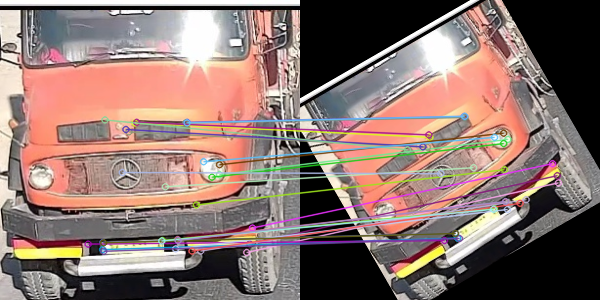
\includegraphics[width=0.9\linewidth]{../assets/matches.png}
  \end{center}
  \vspace{2pt}
  Same car, rotated \& scaled. ORB features still match — lines connect the same physical points.
  This is \term{invariance} working on real data.
\end{frame}

\begin{frame}{How matching works}
  \begin{itemize}
    \item For each descriptor in image A, find the \term{nearest} descriptor in image B (by distance).
    \item Float descriptors (SIFT): Euclidean distance. Binary (ORB): \term{Hamming} distance.
    \item \term{Brute-force} compares all pairs; \term{FLANN} approximates it fast for large sets.
  \end{itemize}
  \begin{mathbox}
    Hamming distance = number of differing bits — a single fast XOR+popcount for binary descriptors.
  \end{mathbox}
\end{frame}

\begin{frame}{Rejecting bad matches}
  \begin{itemize}
    \item Many nearest-neighbour matches are wrong. Filter them:
    \item \term{Ratio test} (Lowe): keep a match only if the best is much closer than the 2nd-best.
    \item \term{Cross-check}: keep only mutual nearest neighbours. \term{RANSAC} (Week 11): reject geometric outliers.
  \end{itemize}
  \begin{badbox}
    Raw matches are noisy. Without the ratio test / RANSAC, a few wrong matches wreck the alignment.
  \end{badbox}
\end{frame}

% ==================================================================
\section{In-class exercise}
% ==================================================================

\begin{frame}{\faPen~In-class exercise (10 min)}
  \begin{infobox}[Reason about invariance]
  \end{infobox}
  \begin{enumerate}
    \item Why is a corner a better feature than a point in the middle of a flat wall?
    \item You match a template plate to a photo taken at an angle and half the size. Which
          descriptor property makes this possible?
    \item After matching, some lines cross wildly (obviously wrong). How do you remove them?
  \end{enumerate}
\end{frame}

\begin{frame}{\faPen~Debrief}
  \begin{itemize}
    \item (1) A corner changes in \emph{all} directions $\rightarrow$ uniquely localizable; a flat point is ambiguous.
    \item (2) \term{Scale and rotation invariance} — the descriptor is the same despite size/angle change.
    \item (3) Ratio test + cross-check remove most; \term{RANSAC} (Week 11) removes geometric outliers by fitting a transform.
  \end{itemize}
  \keyidea{Good features + good matches + outlier rejection = reliable correspondence, the basis of alignment.}
\end{frame}

% ==================================================================
\section{Deep dive}
% ==================================================================

\begin{frame}{Scale invariance: the pyramid}
  \begin{itemize}
    \item To find features at any size, build an \term{image pyramid} (progressively smaller copies).
    \item Detect features at each scale; the scale where a feature is strongest is its ``characteristic scale.''
    \item That's how SIFT/ORB match a small template to a large photo.
  \end{itemize}
\end{frame}

\begin{frame}{How many matches do you need?}
  \begin{itemize}
    \item To estimate a \term{homography} (Week 11) you need $\geq 4$ good correspondences.
    \item In practice, gather dozens of matches, then let \term{RANSAC} pick a consistent set of 4+.
    \item More good matches $\rightarrow$ a more stable, accurate transform.
  \end{itemize}
  \keyidea{Quantity gives robustness: many matches let outlier rejection succeed even when a third are wrong.}
\end{frame}

\begin{frame}{Applications of features}
  \begin{itemize}
    \item \term{Image stitching} (panoramas): match features, find the transform, blend.
    \item \term{Object recognition}: match a template's features to a scene.
    \item \term{Tracking, SLAM, AR}: follow features across video to estimate motion.
    \item \term{DocScan}: match the page/template to align and rectify (Week 11).
  \end{itemize}
\end{frame}

\begin{frame}{Classical features vs deep features}
  \begin{itemize}
    \item Classical (SIFT/ORB): hand-designed, interpretable, no training — still excellent for geometry.
    \item Deep (learned descriptors, SuperPoint): better under extreme appearance change, need training.
    \item For alignment/geometry, classical features remain a strong, practical choice.
  \end{itemize}
  \keyidea{Features are how a computer says ``this point here is the same as that point there'' — the foundation of geometric vision.}
\end{frame}

\begin{frame}[fragile]{Features in code}
\begin{lstlisting}[language=Python]
orb = cv2.ORB_create(500)
kp1, des1 = orb.detectAndCompute(img1, None)
kp2, des2 = orb.detectAndCompute(img2, None)
bf = cv2.BFMatcher(cv2.NORM_HAMMING, crossCheck=True)
matches = sorted(bf.match(des1, des2), key=lambda m: m.distance)
# next week: cv2.findHomography(pts1, pts2, cv2.RANSAC) to align
\end{lstlisting}
  Detect $\rightarrow$ describe $\rightarrow$ match $\rightarrow$ (Week 11) estimate the transform.
\end{frame}

% ==================================================================
\section{Wrap-up}
% ==================================================================

\begin{frame}{What you should now be able to do}
  \begin{itemize}
    \item Explain what makes a good feature (distinctive, repeatable, local) and why corners.
    \item Detect corners (Harris/FAST) and compute descriptors (SIFT/ORB).
    \item Match descriptors; reject bad matches with the ratio test/cross-check.
    \item Understand scale/rotation invariance and the role in alignment.
  \end{itemize}
\end{frame}

\begin{frame}{This week's deliverable}
  \begin{alertblock}{Due before Week 11 (see \code{project/})}
    \begin{enumerate}
      \item Detect Harris corners and ORB keypoints on real images; visualize.
      \item Match ORB features between an image and a rotated/scaled copy; count good matches.
      \item Apply the ratio test / cross-check; show how it removes wrong matches.
      \item Note: how will feature matching help align a photographed page in DocScan?
    \end{enumerate}
  \end{alertblock}
\end{frame}

\begin{frame}[standout]
  Features are ``the same point, seen again.''\\[4pt]
  \normalsize Detect distinctive points, describe them invariantly, match across images.
\end{frame}

\end{document}
